\chapter{Background}
Rather than assume you are familiar with the various concepts or leave you to trawl external sources this chapter aims to provide sufficient background about fundamental aspects needed to understand the domain / context of the research. Some of the concepts and terms I use in the rest of my thesis may be explained here.

\section{Conceptual Model of Apps and App Stores}
The research is situated in apps that are available in app stores. App stores house millions of apps and serve billions of users. They also present a rich tapestry of perspectives on software apps and the ecosystem. There has been a great deal of research that focus on particular areas of these apps and sometimes connect these areas as part of the research. My research focuses on an area seldom investigated, namely it focuses on the developer's view of how their app is perceived by the app store.

\begin{figure}[ht]
    \centering
    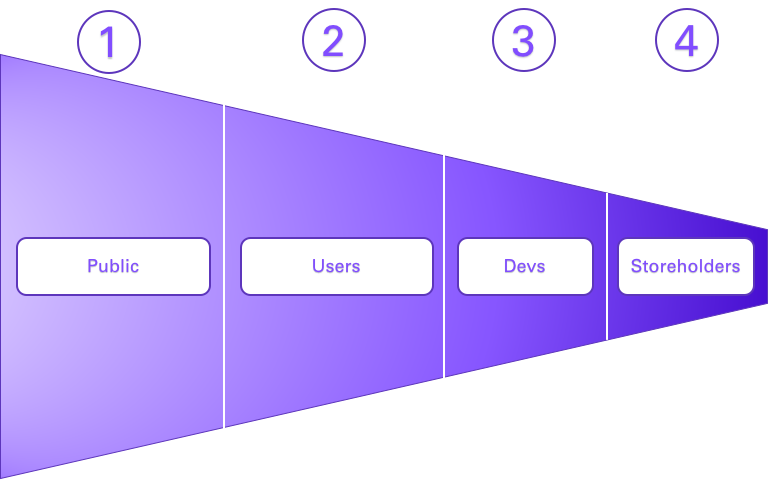
\includegraphics[width=12cm]{images/4-views-of-apps-in-app-store.png}
    \caption{Four Views of an App Store}
    \label{fig:4-views-of-apps-in-app-store}
\end{figure}

Figure~\ref{fig:4-views-of-apps-in-app-store} illustrates the four views. These start from the public view of the app store, what is visible to someone who is not actively engaged with the app store. Examples include people who are not logged into their account, search engines, researchers mining the app store for ratings and reviews, and so on. The public is able to see aggregate ratings and some recent reviews for specific apps. Older reviews are generally hidden from public view (which may limit some research and search engine insights).

The next view is that of a user of a particular app, they have the ability to interact with the app store to rate and review the app. They can see, create, and update their ratings and reviews~\footnote{If supported by the app store, for instance Google Play does.}. They can also see the public view.

Developers have the next view, which includes information the app store records about their interactions with the app store, and information the app store provides the developers directly (\emph{i.e.} generated by the app store and related entities), as well as feedback provided by users via the app store (\emph{e.g.} ratings and reviews). Developers can also see the public view, they cannot see the entire view of their user-base, however they can see any rating and reviews provided by the users.

Both the users and the developers can often see individual ratings and reviews for much longer periods than presented in the public view. 

The final view is that of the app store, the `storeholders' in the figure. They have a global and holistic view of the entire store, including potentially all the reviews, user interactions, and whatever usage activities have been performed by all the other three views.


\section{Three layers of an app}
\begin{figure}[ht]
    \begin{minipage}{\textwidth}
    \centering
    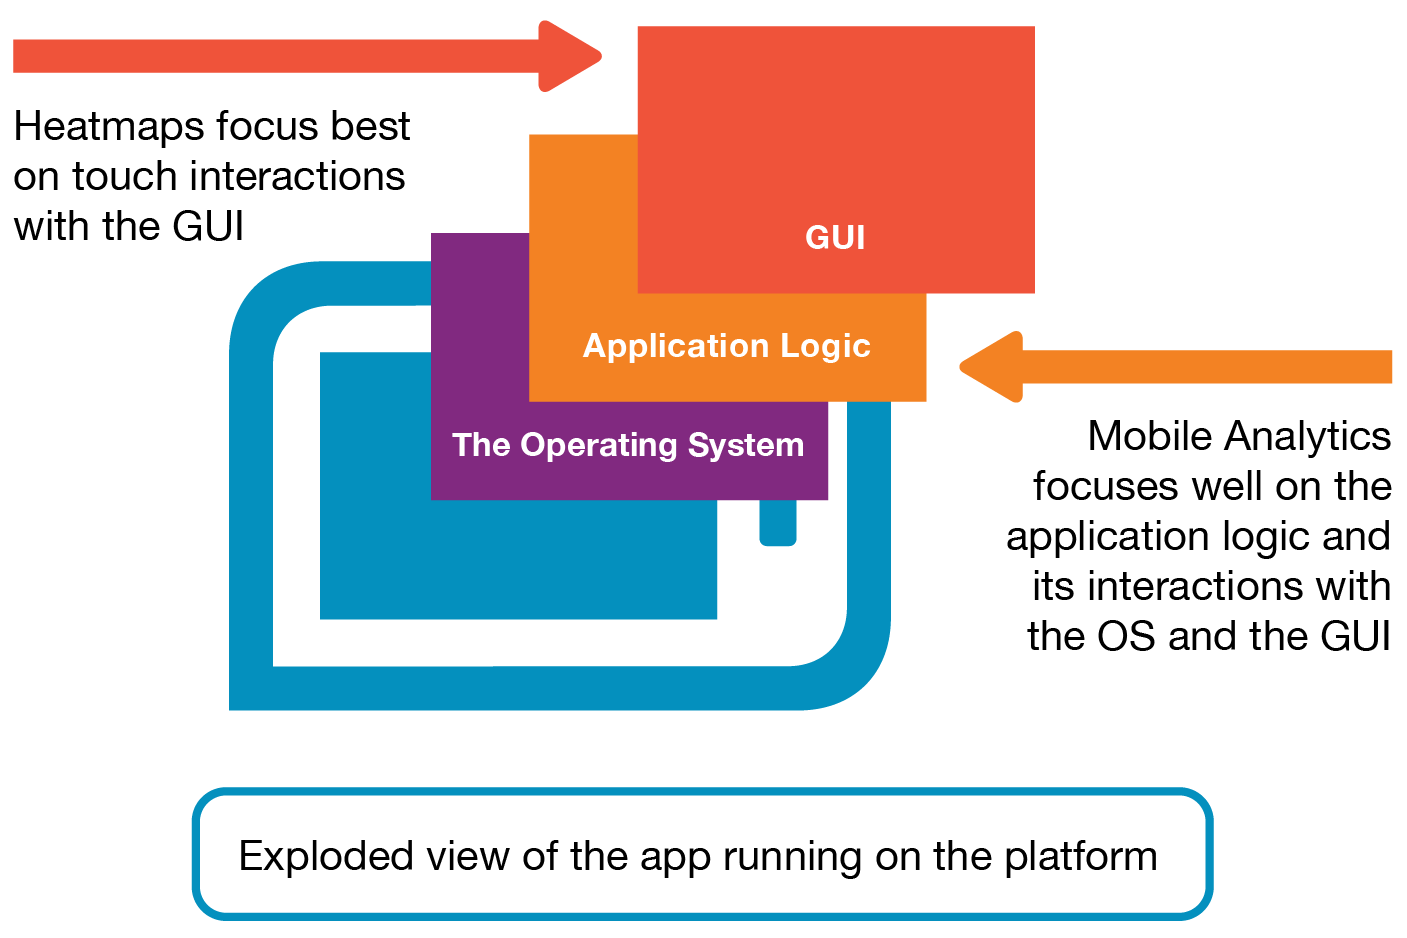
\includegraphics[width=10cm]{images/mobile-analytics-playbook/3-layers.png}
    \caption[Three layers of an app]{Three layers of an app~\footnote{Image credit: First published in the Mobile Analytics Playbook~\cite{harty_aymer_playbook_2016}}.}
    \label{fig:3-layers}
    \end{minipage}
\end{figure}

Figure \ref{fig:3-layers} illustrates three primary observation points, or layers, for a mobile app. 

The Graphical User Interface (GUI) % SHOULD-DO add to glossary.
can be visually observed by sighted users, it can also be observed by Accessibility software, and test automation tools, \emph{etc.} externally to the app. It can also be observed from within the app, for instance through using software known as \emph{heatmapping} that records the screens and the touch interactions performed by users of that screen. One of the the more popular, mature heatmapping offerings is from AppSee~\footnote{\url{  https://www.appbrain.com/stats/libraries/details/appsee/appsee}. Note: in 2019 Appsee's team was acqui-hired by ServiceNow~\url{https://techcrunch.com/2019/05/13/servicenow-acquihires-mobile-analytics-startup-appsee/} and the service no longer directly available.}, nonetheless they are only used in a small minority of mobile apps.


\section{Conceptual Model of Usage Analytics}
Conceptually there appear to be four broad layers of usage analytics, these are illustrated in Figure \ref{fig:four-layers-of-analytics-for-mobile-apps} and described next. They will be discussed in more detail in the  chapter titled~\href{chapter-applying-analytics-to-development-practices}{\emph{\nameref{chapter-applying-analytics-to-development-practices}}}. %MUST_DO decide whether layer and level are synonymous, and if not whether to use one term or the other. Anyway I'm aware I may be conflating both terms here and want to improve the precision of whichever term(s) I use. 

\begin{figure}[ht]
    \centering
    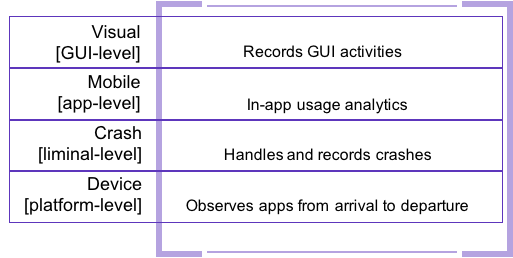
\includegraphics[width=12cm]{images/4-layers-of-analytics.png}
    \caption{Four Layers of Analytics for Mobile Apps}
    \label{fig:four-layers-of-analytics-for-mobile-apps}
\end{figure}

\begin{itemize}
    \item \textbf{Visual (GUI-level)} operates at the GUI level, or layer, of the app. It records aspects of the GUI activities such as touches, gestures, interactions with the screen, and data entry. Often it includes recording what is on the screen too. A common type of Visual analytics is \emph{heatmapping} software.
    \item \textbf{Mobile (app-level)} is incorporated as part of the app and records aspects of what the app is doing, in effect aspects of the usage of the app. Mobile Analytics is prevalent in Android apps and already used for various business purposes.
    \item \textbf{Crash (liminal-level)} is where specialised reporting can intercept crashes. Through the interception they can change the behaviour of the app, for instance to provide a better user-experience, log, and report the crash to the developers. \emph{Fatal crashes} are ones where the application quits. These can also be observed by the operating system; for mobile apps the operating system is an intrinsic part of the platform.
    \item \textbf{Device (platform-level)} Platform-level analytics can record apps from when they are installed until they are removed. This recording can include details such as when apps are in-use, crashes, freezes, and so on. Both of the dominant platforms (iOS and Google Android) allow users to decide whether their devices will share this data.
\end{itemize}


My research includes case studies and developer reports of examples of analytic tools that cover three of these four layers of analytics. The remaining layer, visual analytics, is described briefly with a few examples, visual analytics is seldom used in production mobile apps and therefore I decided to exclude these libraries from my core research. They may be an interesting topic for future research particularly given some of the potential benefits of visual analytics. % COULD_DO add notes on privacy issues and other complicating factors in this sort of research. 


\section{Information sources for app developers}
Developers want and need to know how well their apps are performing from various perspectives such as: growth and adoption (\emph{``do we have more users and are they using the app [more] often?"}), users' ratings and reviews (\emph{``do they like our work?"} and in terms of quality (\emph{``does it perform well? is it fast and reliable?"}). 

\begin{figure}[ht]
    \centering
    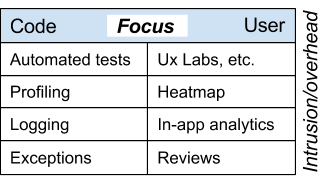
\includegraphics{images/ComparingTechniquesRHS.png}
    \caption{Comparing Techniques}
    \label{fig:comparing_techniques}
\end{figure}

There are various techniques that can be used to assess aspects of quality of mobile apps. Figure \ref{fig:comparing_techniques} provides a visual overview of eight techniques. Of these four are code-oriented and the remaining four more user- or usage- oriented. They are ordered in approximate rank of the overhead, effort, or intrusion involved of each technique. % MUST_DO continue and expand this argument. Discuss why exceptions were chosen as one of the core elements of my research and PhD thesis.

Google's Google Play app store provides developers with answers to all these niggling questions through a developer-oriented user interface called Google Play Console. 
In Google Play Console they provide various tools, reports and data all aimed at informing developers about how their apps are 'doing' and performing. Broadly, these include an overview page with one line of pre-selected data per app managed by the Google Play \textit{Developer Account}. Then, per app, Google provides an overview dashboard of graphs which, in turn, link to more detailed reports and information which provide greater depth. (Examples are provided in the~\href{chapter-analytics-tools}{\emph{\nameref{chapter-analytics-tools}}} chapter.)  Some graphs only appear when Google's algorithms decide they are relevant, these seem to be related to events and/or volumes of underlying data.

\section{Mobile app development lifecycle}
To provide some context for this section, Figure \ref{fig:ci-cd-development-and-feedback}~\footnote{Reproduced from \emph{``An empirical study of architecting for continuous delivery and deployment"}~\cite{shahin2019empirical_study_architecting_cd}}
illustrates a modern continuous software lifecycle including feedback. We can observe several distinct stages in the development and deployment of software and the feedback each stage can provide. %MUST_DO check the guidelines for reproducing and citing a figure as-is.

In contrast, Figure \ref{fig:google-play-app-development-and-feedback} illustrates a similar software lifecycle for Android apps released through Google Play together with the various forms of feedback~\footnote{Here we have excluded feedback from the app store, nonetheless it exists for many app stores.} 

Key differences between typical CI/CD lifecycles and the one for Google Play is the pre-launch testing and the app store providing both user feedback and a service called Android Vitals. The pre-launch reports are generated automatically by Google where the app store runs automated monkey testing on a farm of Android devices and various static analysis checks of releases deployed to any of the test channels. I will explain test channels later on. %MUST_DO actually add information on the test channels and how releases can be promoted to production releases in Google Play.

There are additional sources of \emph{analogue feedback} from people, including from alpha and beta testers and end users; and \emph{digital feedback} from Google tools and from usage data collected from the field. These terms are expanded in the following section~\href{analogue-and-digital-feedback}{\emph{\nameref{analogue-and-digital-feedback}}}.


\begin{figure}[ht]
    \centering
    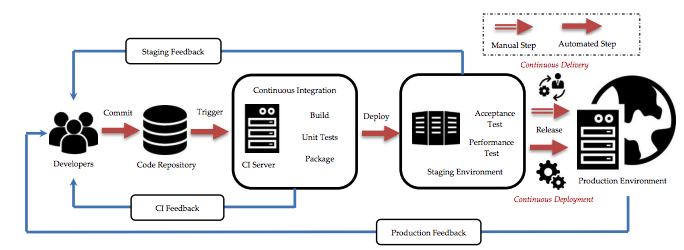
\includegraphics[width=13cm]{images/ci-cd-development-and-feedback.png}
    \caption{CI/CD development and feedback, reproduced from~\cite{shahin2019empirical_study_architecting_cd}}
    \label{fig:ci-cd-development-and-feedback}
\end{figure}

\begin{figure}
    \centering
    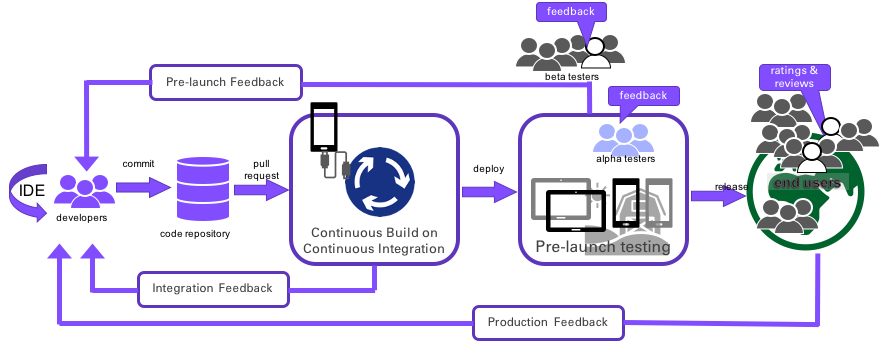
\includegraphics[width=13cm]{images/google-play-app-development.png}
    \caption{Google Play App Development and Feedback}
    \label{fig:google-play-app-development-and-feedback}
\end{figure}


\section{Mobile app usage lifecycle}
Mobile apps have a usage lifecycle, which starts when an app is chosen to be installed and ends with either abandonment or active removal of the app from a device. Figure~\ref{fig:mobile_app_usage_lifecycle}~\footnote{Based on a figure in~\cite{bohmer2011falling_asleep_with_angry_birds}} illustrates the possible stages of a mobile app's life on a user's device.

\begin{figure}[ht]
    \centering
    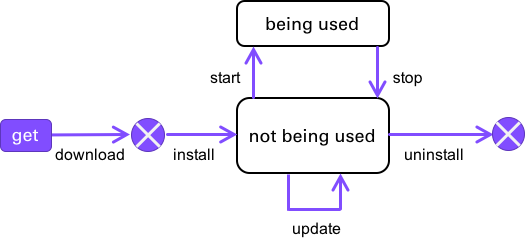
\includegraphics[width=12cm]{images/mobile_app_usage_lifecycle.png}
    \caption{Mobile App Usage Lifecycle}
    \label{fig:mobile_app_usage_lifecycle}
\end{figure}

A later section~\href{platform-level-analytics}{\emph{\nameref{platform-level-analytics}}} provides details of my understanding of how Google collects the underlying data (they do not document, explain or encourage research in how their system works, We return to their behaviour and the effects later in this introduction). And the chapter \href{chapter-software-we-developed-for-google-play-console}{\emph{\nameref{chapter-software-we-developed-for-google-play-console}}} describes software we developed to help collect data from Google Play Console in order to facilitate both research and to enable developers to collect and use data...

Crashes are often considered a concrete measure of poor performance of software and there has been extensive research in crashes for Android applications, in particular. I suspect there are various reasons for the focus on crashes as an oracle for testing software, crashes are unambiguous (even if the causes are not) and they are also binary so easy to determine whether software has, or has not, crashed. 

Google launched a service called Android Vitals as a new, intrinsic part of Google Play Console in 2016/17 \emph{TODO confirm the date and revise this sentence} where they popularised a measure called \emph{Stability} to assess the quality of Android apps. Their measure includes both crashes and when an application freezes or is unresponsive for at least 5 seconds from a user's perspective, a term Google call Application Not Responding (ANR).

\section{Analogue and Digital Feedback}~\label{analogue-and-digital-feedback}
Feedback can help developers to find and choose ways to improve their software. Various researchers have investigated way to understand and use feedback provided by end-users, for instance, in ratings and reviews users provide to the app store. For the purposes of my research I term feedback people provide as \emph{analogue feedback} as it has the richness and complexity of analogue signals, and also challenges of processing and comprehension.

In contrast, digital feedback originates from software and is generally deterministic~\footnote{~\url{https://en.wiktionary.org/wiki/deterministic}}. For the purposes of my research I consider digital feedback as that provided by running software where programmers added code to programs to collect data that provides feedback about software use and certain behaviours of that software. The addition of the code may be automated, in part, or wholly, for instance by another program or script. As an example, AppPulse Mobile claims they can add analytics automatically without developers writing a line of code~\footnote{~\url{https://www.microfocus.com/en-us/products/apppulse-mobile-app-apm-monitoring/overview}}.

\begin{figure}[ht]
    \centering
    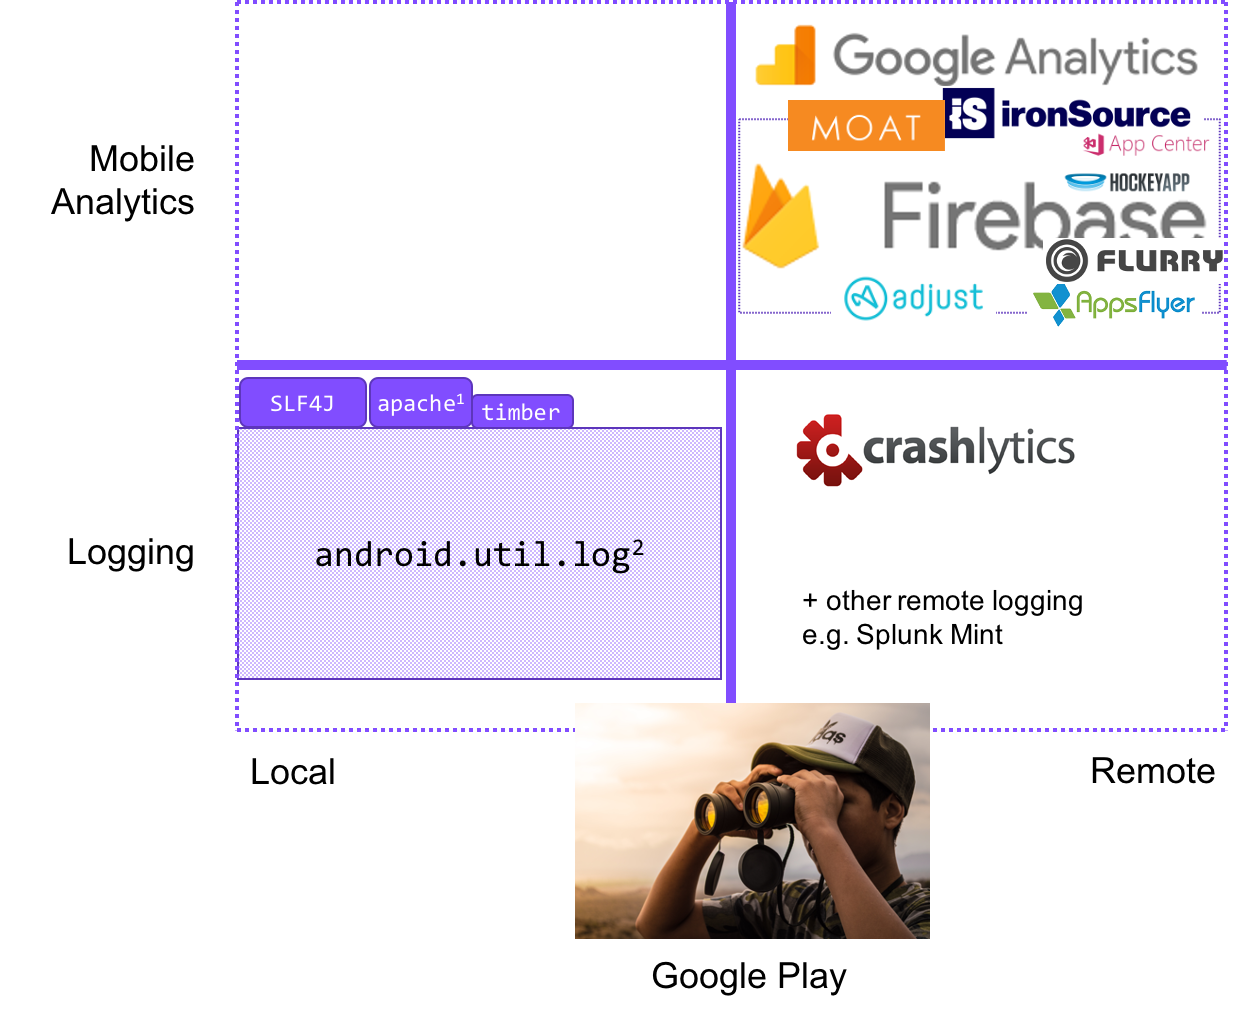
\includegraphics[width=12cm]{images/matrix-of-logging.png}
    \caption{Matrix of logging}
    \label{fig:matrix-of-logging}
\end{figure}

The application may incorporate logging and/or mobile analytics. Logging in mobile apps is often used locally, by developers independently of other mechanisms. Figure \ref{fig:matrix-of-logging} illustrates a matrix of logging, where logging and mobile analytics are on the Y axis and local and remote on the X axis. Google Play is an external observer of data recorded in device logs. Data collection runs locally and is sent to Google servers where Google analyses the data and provides reports to developers for their apps.

As an observation the vast majority of Android developers use the default inbuilt logging library \texttt{android.util.log} and choose one or more of Google's analytics offerings (which include Firebase and Crashlytics). A commercial organisation provides current statistics for third-party logging libraries~\footnote{Logging libraries (note the default library is not tracked at the time of writing~\url{https://www.appbrain.com/stats/libraries/tag/logging/logging-libraries}}, crash libraries~\footnote{\url{https://www.appbrain.com/stats/libraries/tag/crash-reporting/android-crash-reporting-libraries}} and mobile analytics~\footnote{\url{https://www.appbrain.com/stats/libraries/tag/analytics/android-analytics-libraries}}. Some apps have several of these libraries so counts may exceed 100\% in their reports.

\begin{itemize}
    \item Logging: enables developers to understand what their software is doing. The practice is commonplace across many software domains including mobile apps, and each platform and language includes a standard method of generating log messages. These messages tend to be small and intended for immediate, local consumption. On Android when developers use the standard logging library (\texttt{android.util.log}) their log messages are written to a shared circular log file on a device. Some privileged Android software is able to read these shared logs, developers can also read them using standard Android development tools \emph{e.g.} \texttt{adb logcat} providing they are connected to the device with the log file. Older versions of Android allowed apps to read the full contents, more recently apps are restricted to only the log messages they wrote unless they are granted the relevant permission by Google and the user. 
    In other domains \emph{e.g.} web servers, infrastructure software, and many others, logging is used for production monitoring, fault-finding and analysis. A minority of mobile app developers use remote logging.
    \item Mobile analytics, can extend and scale logging. For mobile analytics, a minority of developers incorporate custom implementations, however the vast majority who use analytics do so through using third-party analytics libraries such as Google Firebase Analytics, details of the current usage of analytics libraries are provided by AppBrain~\footnote{\url{https://www.appbrain.com/stats/libraries/tag/analytics/android-analytics-libraries}}.
\end{itemize}

Similar to the concept of black box testing (where software's behaviour is observed and assessed without knowing the internals), external software can observe the behaviours of apps. Google have developed and integrated software that monitors apps running in Google approved versions of Android. The data is collected per device and provided automatically to Google servers if the device has the relevant settings enabled~\cite{google_play_share_usage_and_diagnostics_info_with_google}. This data is processed by Google who provide some portions of the data to the registered developers of that app in the Google Play Store.

\emph{Idea for expansion:} Drop-off in data for a population  c.f. marketing funnels, funnels for shopping carts, etc.

% Mobile Developer's Guide to the fifth dimension
% available from https://www.dropbox.com/s/no70z2hiod6z7o8/Fifth_Dimension_v1.pdf?dl=0 (took 20 - 30 mins to track down)

\section{Active and passive analytics choices}
Various degrees of choices are available depending on how actively the development team wish to incorporate analytics into their development practices. These include using what already exists, where the data is gathered by others and made available to the developers, here these sources are called \emph{passive analytics}. Developers can choose to take more authority in the data collection, for instance by deciding what data they would like to collect and how the wish to collect it. They can use these tools at various depths, ranging from superficial use to actively maximising the efficacy of using analytics to provide them with the data they believe they need to achieve their outcomes.

\subsection{Passive Analytics}~\label{subsection-passive-analytics}
Passive analytics are those not actively under the control or influence of the development team, they are provided from other sources such as the operating system or the app store. In my research the passive analytics are all managed by the app store, Google Play Console.



\section{An aside on packaging mobile apps}~\label{section-packaging-mobile-apps}
Mobile apps are a bit like snails, who carry everything with them in their shell, well actually in their application binary package (known as an APK~\footnote{Android Package Kit\url{https://en.wikipedia.org/wiki/Android_application_package}} file). This includes whichever libraries they use. Therefore, when developers want to include pre-packaged support for crash-reporting and/or mobile analytics, the development team need to incorporate the relevant software libraries in their application binary package. These libraries are therefore distributed as an intrinsic part of an app and installed seamlessly with the main application onto a user's device.


\subsection{The Reaper Cometh}
AppBrain is a business that actively monitors and reports on Android Apps in the Google Play Store. The business was founded by two ex-Google engineers, as I am. They state Google is actively culling Android apps from the Google Play store and estimate approximately 16\% of apps are \emph{"low quality apps"} and \emph{"unlikely to be useful"}~\footnote{\url{https://www.appbrain.com/stats/number-of-android-apps}} % Percentage of low quality apps: 16%

